\begin{figure}[ht]
    \centering
    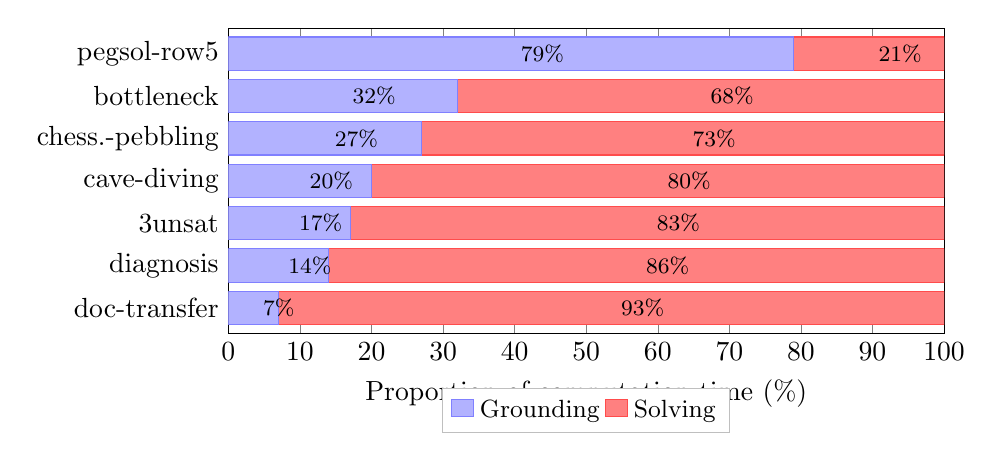
\begin{tikzpicture}
        \begin{axis}[
                xbar stacked,
                width=0.88\textwidth,
                height=0.45\textwidth,
                xlabel={Proportion of computation time (\%)},
                xmin=0, xmax=100,
                ytick=data,
                yticklabels={
                        pegsol-row5,
                        bottleneck,
                        chess.-pebbling,
                        cave-diving,
                        3unsat,
                        diagnosis,
                        doc-transfer},
                y dir=reverse,
                legend style={
                        font=\small,
                        at={(0.5,-0.18)},
                        anchor=north,
                        draw=gray!50,
                    },
                legend columns=2,
                bar width=12pt,
                nodes near coords={\pgfmathprintnumber{\pgfplotspointmeta}\%},
                nodes near coords align={horizontal},
                every node near coord/.append style={font=\footnotesize},
            ]
            % Grounding portion (first stack segment)
            \addplot[fill=blue!30, draw=blue!50] coordinates {
                    (79,0) (32,1) (27,2) (20,3) (17,4) (14,5) (7,6)
                };
            \addlegendentry{Grounding}
            % Solving portion (second stack segment)
            \addplot[fill=red!50, draw=red!70] coordinates {
                    (21,0) (68,1) (73,2) (80,3) (83,4) (86,5) (93,6)
                };
            \addlegendentry{Solving}
        \end{axis}
    \end{tikzpicture}
    \caption{Median proportion of grounding-plus-solving time spent in each phase, per domain. Solving dominates in six of seven domains; only \textit{pegsol-row5} is grounding-dominated. Translation and extraction are omitted ($<\!1\%$ in all cases).}
    \label{fig:phase_proportions}
\end{figure}
